\chapter{Fundamentos de optimización}
\label{cap:optimizacion}

Entrenar un modelo es resolver un problema de optimización: encontrar los parámetros $\vth$ que hacen
mínima una función de pérdida $J(\vth)$. Elegir un umbral de detección con una tasa de falsas alarmas
fija también lo es, pero con una restricción. Este capítulo reúne la teoría que se usa en el resto del
trabajo: óptimos locales y globales, convexidad, descenso por gradiente, multiplicadores de Lagrange,
condiciones de Karush-Kuhn-Tucker (KKT), dualidad, el simplex y la programación lineal. Al final se aplica
a tres problemas concretos del trabajo: la función softmax, el dual del SVM y el umbral de
Neyman-Pearson. La referencia principal es \textcite{boyd2004}; para los algoritmos, \textcite{nocedal2006}.

\section{Planteo general}

El problema de optimización en su forma general es
\begin{equation}
  \min_{\vth \in \R^d}\ f_0(\vth)
  \quad\text{sujeto a}\quad
  f_i(\vth) \le 0,\ i = 1,\dots,m, \qquad h_j(\vth) = 0,\ j = 1,\dots,p.
  \label{eq:problema_general}
\end{equation}
$f_0$ es la \emph{función objetivo}; las $f_i$ y $h_j$ definen el \emph{conjunto factible}
$\mathcal{D} = \{\vth : f_i(\vth) \le 0,\ h_j(\vth) = 0\}$. Maximizar $g$ es lo mismo que minimizar $-g$, así
que basta con estudiar la minimización. Si no hay restricciones, el problema es \emph{irrestricto}: es el
caso del entrenamiento de la regresión logística y de la red convolucional.

\section{Óptimo local y global}
\label{sec:local_global}

\begin{definicion}
Sea $J : \mathcal{D} \to \R$. Un punto $\vth^* \in \mathcal{D}$ es
\begin{itemize}
  \item \textbf{mínimo global} si $J(\vth^*) \le J(\vth)$ para todo $\vth \in \mathcal{D}$;
  \item \textbf{mínimo local} si existe $\varepsilon > 0$ tal que $J(\vth^*) \le J(\vth)$ para todo
        $\vth \in \mathcal{D}$ con $\lVert \vth - \vth^* \rVert < \varepsilon$;
  \item mínimo local o global \textbf{estricto} si la desigualdad es estricta para $\vth \neq \vth^*$.
\end{itemize}
\end{definicion}

Todo mínimo global es local; la recíproca es falsa en general. Un algoritmo que usa solo información
local (el valor de $J$ y de sus derivadas en el punto actual, como todos los que se usan en este trabajo)
no tiene forma de distinguir un mínimo local de uno global: si llega a un mínimo local, se queda ahí.

\subsection{Condiciones de optimalidad sin restricciones}

\begin{teorema}[Condición necesaria de primer orden]
\label{teo:primer_orden}
Si $J$ es diferenciable y $\vth^*$ es un mínimo local de $J$ en $\R^d$, entonces $\nabla J(\vth^*) = \mathbf{0}$.
\end{teorema}
\begin{proof}
Sea $\mathbf{d} = -\nabla J(\vth^*)$. Por la definición de derivada,
$J(\vth^* + t\mathbf{d}) = J(\vth^*) - t\lVert\nabla J(\vth^*)\rVert^2 + o(t)$. Si el gradiente no fuera nulo,
para $t > 0$ suficientemente chico se tendría $J(\vth^* + t\mathbf{d}) < J(\vth^*)$, lo que contradice que
$\vth^*$ es un mínimo local.
\end{proof}

Un punto con gradiente nulo se llama \emph{punto estacionario} o \emph{crítico}. Puede ser un mínimo, un
máximo o un \emph{punto silla}. Para distinguirlos hacen falta las derivadas segundas.

\begin{teorema}[Condiciones de segundo orden]
\label{teo:segundo_orden}
Sea $J$ dos veces diferenciable con continuidad y $\nabla J(\vth^*) = \mathbf{0}$.
\begin{enumerate}
  \item (Necesaria) Si $\vth^*$ es mínimo local, la Hessiana $\nabla^2 J(\vth^*)$ es semidefinida positiva.
  \item (Suficiente) Si $\nabla^2 J(\vth^*)$ es definida positiva, $\vth^*$ es un mínimo local estricto.
\end{enumerate}
\end{teorema}
\begin{proof}
Por el desarrollo de Taylor de segundo orden alrededor de un punto con gradiente nulo,
\[
  J(\vth^* + \mathbf{v}) = J(\vth^*) + \tfrac12\, \mathbf{v}^\top \nabla^2 J(\vth^*)\, \mathbf{v} + o(\lVert\mathbf{v}\rVert^2).
\]
(1) Si existiera $\mathbf{v}$ con $\mathbf{v}^\top \nabla^2 J\,\mathbf{v} < 0$, tomando $t\mathbf{v}$ con $t$ chico la
función bajaría, contradicción. (2) Si $\nabla^2 J \succ 0$, su menor autovalor $\mu$ es positivo y
$\mathbf{v}^\top\nabla^2 J\,\mathbf{v} \ge \mu\lVert\mathbf{v}\rVert^2$; para $\mathbf{v}$ chico el término
$o(\lVert\mathbf{v}\rVert^2)$ es menor que $\tfrac{\mu}{2}\lVert\mathbf{v}\rVert^2$, así que
$J(\vth^* + \mathbf{v}) > J(\vth^*)$.
\end{proof}

Estas condiciones son \emph{locales}: certifican que no hay nada mejor en un entorno de $\vth^*$, pero no
dicen nada sobre el resto del espacio. La convexidad es la propiedad que permite pasar de local a global.

\section{Conjuntos y funciones convexas}
\label{sec:convexidad}

\begin{definicion}
Un conjunto $\mathcal{D} \subseteq \R^d$ es \textbf{convexo} si para todo $\vth_1, \vth_2 \in \mathcal{D}$ y
$t \in [0,1]$, el punto $t\vth_1 + (1-t)\vth_2$ pertenece a $\mathcal{D}$. Una función $J : \mathcal{D} \to \R$,
con $\mathcal{D}$ convexo, es \textbf{convexa} si
\begin{equation}
  J\big(t\vth_1 + (1-t)\vth_2\big) \le t\,J(\vth_1) + (1-t)\,J(\vth_2)
  \qquad \forall\, \vth_1, \vth_2 \in \mathcal{D},\ t \in [0,1],
  \label{eq:def_convexa}
\end{equation}
y \textbf{estrictamente convexa} si la desigualdad es estricta cuando $\vth_1 \ne \vth_2$ y $t \in (0,1)$.
\end{definicion}

Geométricamente, la cuerda entre dos puntos del gráfico queda por encima del gráfico. Ejemplos que
aparecen en el trabajo: las normas $\lVert\vth\rVert$ y $\lVert\vth\rVert^2$, las funciones afines (convexas y
cóncavas a la vez), $\log(1 + e^z)$, la función \emph{log-sum-exp} $\log\sum_k e^{z_k}$ y la pérdida bisagra
$\max(0, 1 - z)$. Los poliedros $\{\vth : A\vth \le \mathbf{b}\}$ y el simplex
(Sección~\ref{sec:simplex}) son conjuntos convexos.

\begin{proposicion}[Caracterizaciones con derivadas]
\label{prop:caracterizacion}
Sea $J$ diferenciable en un dominio convexo abierto.
\begin{enumerate}
  \item $J$ es convexa si y solo si $J(\vth_2) \ge J(\vth_1) + \nabla J(\vth_1)^\top(\vth_2 - \vth_1)$ para todo
        $\vth_1, \vth_2$: el plano tangente queda siempre por debajo del gráfico.
  \item Si $J$ es dos veces diferenciable, $J$ es convexa si y solo si $\nabla^2 J(\vth) \succeq 0$ en todo
        punto. Si $\nabla^2 J(\vth) \succ 0$ en todo punto, $J$ es estrictamente convexa.
\end{enumerate}
\end{proposicion}

La condición (1) tiene una consecuencia inmediata: si $\nabla J(\vth^*) = \mathbf{0}$ y $J$ es convexa,
entonces $J(\vth) \ge J(\vth^*)$ para \emph{todo} $\vth$. Es decir, en una función convexa diferenciable
\emph{la condición de primer orden ya es suficiente para el óptimo global}. El teorema siguiente lo dice
sin pedir diferenciabilidad.

\begin{teorema}
\label{teo:local_global}
Sea $J$ convexa sobre un conjunto convexo $\mathcal{D}$.
\begin{enumerate}
  \item Todo mínimo local de $J$ es un mínimo global.
  \item El conjunto de minimizadores globales es convexo.
  \item Si $J$ es estrictamente convexa, tiene a lo sumo un minimizador.
\end{enumerate}
\end{teorema}
\begin{proof}
(1) Sea $\vth^*$ un mínimo local con radio $\varepsilon$ y supongamos que existe $\tilde\vth \in \mathcal{D}$ con
$J(\tilde\vth) < J(\vth^*)$. Para $t \in (0,1]$ el punto $\vth_t = (1-t)\vth^* + t\tilde\vth$ está en
$\mathcal{D}$ (convexidad del conjunto) y, por la convexidad de $J$,
\[
  J(\vth_t) \le (1-t)\,J(\vth^*) + t\,J(\tilde\vth) < J(\vth^*).
\]
Tomando $t < \varepsilon / \lVert\tilde\vth - \vth^*\rVert$ se tiene $\lVert\vth_t - \vth^*\rVert < \varepsilon$, y
$\vth_t$ es un punto del entorno con menor valor: contradicción.

(2) Si $\vth_1$ y $\vth_2$ son minimizadores con valor $J^*$, cualquier combinación convexa cumple
$J(t\vth_1 + (1-t)\vth_2) \le tJ^* + (1-t)J^* = J^*$, así que también es minimizador.

(3) Si $\vth_1 \neq \vth_2$ fueran dos minimizadores, la convexidad estricta daría
$J(\tfrac12\vth_1 + \tfrac12\vth_2) < J^*$, lo que es imposible.
\end{proof}

\begin{observacion}
El punto (2) da un criterio práctico para \emph{refutar} la convexidad: si se encuentran dos soluciones
$\vth_1, \vth_2$ con la misma pérdida y en su punto medio la pérdida es mayor, la función no es convexa.
Es el experimento que se hace con una red neuronal chica en el Capítulo~\ref{cap:convexos}: dos soluciones
con pérdida 0,041 tienen en su punto medio una pérdida de 0,596.
\end{observacion}

\subsection{Operaciones que preservan la convexidad}

Probar la convexidad desde la definición suele ser engorroso. En la práctica se usan reglas de composición:
\begin{itemize}
  \item La suma de funciones convexas, y el producto por un escalar no negativo, es convexa.
  \item Si $J$ es convexa, $\vth \mapsto J(A\vth + \mathbf{b})$ también lo es (composición con una función afín).
  \item El máximo puntual de funciones convexas es convexo.
\end{itemize}
Con estas reglas, la pérdida logística regularizada
$\frac1n\sum_i \big[\log(1 + e^{\vth^\top\tilde\vx_i}) - y_i\vth^\top\tilde\vx_i\big] + \frac{\lambda}{2}\lVert\vw\rVert^2$
es convexa (suma de convexas compuestas con funciones afines, más un término afín, más una norma al cuadrado),
y lo mismo pasa con el objetivo del SVM, $\frac12\lVert\vw\rVert^2 + C\sum_i\max(0, 1 - y_i(\vw^\top\vx_i + b))$.
En el Capítulo~\ref{cap:convexos} se calcula la Hessiana de la logística y se prueba que es \emph{estrictamente}
convexa.

\subsection{Convexidad fuerte}

\begin{definicion}
$J$ es \textbf{$\mu$-fuertemente convexa} ($\mu > 0$) si $J(\vth) - \frac{\mu}{2}\lVert\vth\rVert^2$ es convexa.
Si $J$ es dos veces diferenciable, equivale a $\nabla^2 J(\vth) \succeq \mu I$ en todo punto, y a
\begin{equation}
  J(\vth_2) \ge J(\vth_1) + \nabla J(\vth_1)^\top(\vth_2 - \vth_1) + \frac{\mu}{2}\lVert\vth_2 - \vth_1\rVert^2.
  \label{eq:fuerte}
\end{equation}
\end{definicion}

Sumar un término de regularización $\frac{\lambda}{2}\lVert\vth\rVert^2$ a una pérdida convexa la vuelve
$\lambda$-fuertemente convexa. Esta es una razón \emph{de optimización}, además de la estadística, para regularizar:
garantiza un único mínimo y una convergencia rápida del descenso por gradiente.

\subsection{Funciones no convexas: las redes neuronales}
\label{sec:no_convexo}

La pérdida de una red neuronal con capas ocultas no es convexa. Hay dos fenómenos distintos:
\begin{enumerate}
  \item \textbf{Simetrías.} Si se permutan las $h$ neuronas de una capa oculta (con sus pesos de entrada y de
        salida), la red calcula exactamente la misma función. Con activación impar ($\tanh$), cambiar el signo
        de los pesos de entrada y de salida de una neurona tampoco cambia nada. Cada mínimo tiene entonces
        $h!\,2^h$ copias con la misma pérdida. Por el Teorema~\ref{teo:local_global}(2), si la función fuera
        convexa también serían mínimos todos los puntos intermedios, y no lo son.
  \item \textbf{Mínimos locales genuinos}, con pérdida peor que la del mínimo global, donde el descenso por
        gradiente puede quedar atrapado. En el Capítulo~\ref{cap:convexos} una red de 2 neuronas termina en 8
        mínimos distintos según la semilla, con pérdidas que varían en un factor 20.
\end{enumerate}
En redes grandes, como la CNN del Capítulo~\ref{cap:cnn}, la evidencia empírica \parencite{goodfellow2016}
indica que la mayoría de los puntos críticos de alta dimensión son puntos silla y no mínimos malos, y que los
mínimos que se encuentran tienen pérdidas de entrenamiento parecidas. Pero la \emph{generalización} de esos
mínimos sí puede diferir, y depende del optimizador y de la tasa de aprendizaje. Por eso la comparación de
optimizadores se hace con varias semillas y se mide sobre pacientes no vistos.

\section{Descenso por gradiente}
\label{sec:gradiente}

El método más simple para minimizar una función diferenciable es moverse en la dirección opuesta al gradiente,
que es la de mayor descenso local:
\begin{equation}
  \vth_{k+1} = \vth_k - \eta\, \nabla J(\vth_k),
  \label{eq:gd}
\end{equation}
con \emph{tasa de aprendizaje} (o paso) $\eta > 0$. La pregunta es qué valor de $\eta$ usar y qué tan rápido
converge.

\begin{algorithm}[ht]
\caption{Descenso por gradiente con paso fijo.}
\label{alg:gd}
\begin{algorithmic}[1]
\Require $J$ diferenciable, punto inicial $\vth_0$, paso $\eta$, tolerancia $\epsilon$
\State $k \gets 0$
\While{$\lVert\nabla J(\vth_k)\rVert > \epsilon$}
  \State $\vth_{k+1} \gets \vth_k - \eta\,\nabla J(\vth_k)$
  \State $k \gets k + 1$
\EndWhile
\State \Return $\vth_k$
\end{algorithmic}
\end{algorithm}

\subsection{Suavidad y elección del paso}

\begin{definicion}
El gradiente de $J$ es \textbf{$L$-Lipschitz} (o $J$ es $L$-suave) si
$\lVert\nabla J(\vth_1) - \nabla J(\vth_2)\rVert \le L\,\lVert\vth_1 - \vth_2\rVert$ para todo par de puntos.
Si $J$ es dos veces diferenciable, equivale a que todos los autovalores de $\nabla^2 J$ estén acotados por $L$
en valor absoluto.
\end{definicion}

\begin{lema}[Lema de descenso]
\label{lem:descenso}
Si $J$ es $L$-suave, para todo $\vth, \vth'$:
\begin{equation}
  J(\vth') \le J(\vth) + \nabla J(\vth)^\top(\vth' - \vth) + \frac{L}{2}\lVert\vth' - \vth\rVert^2.
  \label{eq:descenso}
\end{equation}
En particular, con $\vth' = \vth - \eta\nabla J(\vth)$,
\begin{equation}
  J(\vth') \le J(\vth) - \eta\Big(1 - \frac{L\eta}{2}\Big)\lVert\nabla J(\vth)\rVert^2.
\end{equation}
\end{lema}
\begin{proof}
Por el teorema fundamental del cálculo aplicado a $t \mapsto J(\vth + t(\vth'-\vth))$,
\[
  J(\vth') - J(\vth) - \nabla J(\vth)^\top(\vth'-\vth)
  = \int_0^1 \big[\nabla J(\vth + t(\vth'-\vth)) - \nabla J(\vth)\big]^\top(\vth'-\vth)\,dt
  \le \int_0^1 L\,t\,\lVert\vth'-\vth\rVert^2\,dt = \frac{L}{2}\lVert\vth'-\vth\rVert^2,
\]
usando Cauchy-Schwarz y la condición de Lipschitz. La segunda desigualdad sale de reemplazar
$\vth' - \vth = -\eta\nabla J(\vth)$.
\end{proof}

El lema dice que \emph{cualquier} paso $0 < \eta < 2/L$ hace bajar la función, y que la cota de descenso
es máxima con $\eta = 1/L$:
\begin{equation}
  J(\vth_{k+1}) \le J(\vth_k) - \frac{1}{2L}\lVert\nabla J(\vth_k)\rVert^2.
  \label{eq:descenso_1L}
\end{equation}
Con un paso mayor que $2/L$ el método puede diverger: en una cuadrática con curvatura $L$ en alguna dirección,
cada iteración multiplica el error en esa dirección por $|1 - \eta L| > 1$. Es la versión teórica del
fenómeno que se observa con tasas de aprendizaje altas en la CNN (picos en la curva de validación,
Capítulo~\ref{cap:cnn}).

\subsection{Velocidad de convergencia}

\begin{teorema}
\label{teo:convergencia}
Sea $J$ $L$-suave con mínimo $J^* = J(\vth^*)$ y $\eta = 1/L$.
\begin{enumerate}
  \item Si $J$ es convexa, $J(\vth_k) - J^* \le \dfrac{L\,\lVert\vth_0 - \vth^*\rVert^2}{2k}$ (convergencia sublineal, $O(1/k)$).
  \item Si $J$ es $\mu$-fuertemente convexa,
        \begin{equation}
          J(\vth_k) - J^* \le \Big(1 - \frac{\mu}{L}\Big)^k\,\big(J(\vth_0) - J^*\big)
          \label{eq:lineal}
        \end{equation}
        (convergencia \emph{lineal} o geométrica: el error baja un factor fijo por iteración).
\end{enumerate}
\end{teorema}
\begin{proof}[Demostración de (2)]
Minimizando en $\vth_2$ los dos miembros de~\eqref{eq:fuerte}, con $\vth_1 = \vth_k$: el miembro izquierdo da
$J^*$ y el derecho, una cuadrática en $\vth_2$, alcanza su mínimo en $\vth_2 = \vth_k - \nabla J(\vth_k)/\mu$.
Resulta la desigualdad
\[
  J^* \ge J(\vth_k) - \frac{1}{2\mu}\lVert\nabla J(\vth_k)\rVert^2,
  \qquad\text{o sea}\qquad
  \lVert\nabla J(\vth_k)\rVert^2 \ge 2\mu\big(J(\vth_k) - J^*\big).
\]
Reemplazando en~\eqref{eq:descenso_1L} y restando $J^*$:
$J(\vth_{k+1}) - J^* \le \big(J(\vth_k) - J^*\big) - \frac{\mu}{L}\big(J(\vth_k) - J^*\big)$. Aplicando la
desigualdad $k$ veces se obtiene~\eqref{eq:lineal}.
\end{proof}

La demostración de (1) usa un argumento parecido sumando telescópicamente; puede verse en
\textcite[Sec.~9.3]{boyd2004}. El cociente $\kappa = L/\mu \ge 1$ es el \textbf{número de condición} del
problema: mide cuánto más curvada es la función en su dirección más empinada que en la más plana. Para
reducir el error en un factor $\epsilon$ hacen falta del orden de $\kappa\log(1/\epsilon)$ iteraciones. Con
$\kappa$ grande, el descenso por gradiente avanza en zigzag por un valle angosto; los métodos con momento
del Capítulo~\ref{cap:cnn} reducen esa dependencia a $\sqrt\kappa$.

\paragraph{Ejemplo numérico.} Para la regresión logística binaria de Bonn (ictal contra el resto, 20 atributos
estandarizados más el sesgo, $\lambda = 0{,}01$) la cota de Lipschitz del Capítulo~\ref{cap:convexos} es
$L = \tfrac{1}{4n}\lambda_{\max}(\tilde X^\top\tilde X) + \lambda = 4{,}298$, de modo que se usa
$\eta = 1/L = 0{,}233$. Cerca del óptimo, el menor autovalor de la Hessiana es $\mu \approx 0{,}0081$
(el sesgo no está regularizado, así que la convexidad fuerte es local, no global). El número de condición
efectivo es $\kappa \approx 528$, y la cota~\eqref{eq:lineal} predice un factor $1 - 1/528 \approx 0{,}998$
por iteración: unas 14\,600 iteraciones para reducir la brecha en 12 órdenes de magnitud. Es consistente con
el experimento del Capítulo~\ref{cap:convexos}, donde las 20\,000 iteraciones llevan la brecha hasta la
precisión de punto flotante con una caída lineal en escala logarítmica.

\subsection{Descenso por gradiente estocástico}

Cuando la pérdida es un promedio sobre $n$ ejemplos, $J(\vth) = \frac1n\sum_i \ell_i(\vth)$, calcular el gradiente
completo cuesta $O(n)$. El \emph{descenso estocástico} (SGD) usa en cada paso el gradiente de un \emph{lote}
$\mathcal{B}_k$ de $B$ ejemplos elegidos al azar:
\begin{equation}
  \vth_{k+1} = \vth_k - \eta\,\mathbf{g}_k, \qquad
  \mathbf{g}_k = \frac{1}{B}\sum_{i \in \mathcal{B}_k}\nabla\ell_i(\vth_k), \qquad \E[\mathbf{g}_k] = \nabla J(\vth_k).
\end{equation}
El gradiente estimado es insesgado pero ruidoso, con varianza proporcional a $1/B$. Con paso fijo, SGD no
converge al óptimo exacto sino a un entorno cuyo tamaño crece con $\eta$; para converger hay que reducir el
paso. En redes neuronales ese ruido no es solo un costo: ayuda a escapar de puntos silla y se asocia a mínimos
que generalizan mejor \parencite{wilson2017}. La CNN se entrena con lotes de $B = 64$
(Capítulo~\ref{cap:cnn}).

\section{Multiplicadores de Lagrange}
\label{sec:lagrange}

\subsection{Restricciones de igualdad}

Se busca minimizar $f(\vth)$ sujeto a $h_j(\vth) = 0$, $j = 1,\dots,p$. La idea geométrica: en un mínimo
restringido, moverse a lo largo de la restricción no puede hacer bajar $f$. Las direcciones permitidas
(tangentes) son las $\mathbf{d}$ con $\nabla h_j(\vth^*)^\top\mathbf{d} = 0$ para todo $j$, y en todas ellas
debe ser $\nabla f(\vth^*)^\top\mathbf{d} = 0$. Eso dice que $\nabla f(\vth^*)$ es ortogonal al espacio tangente,
es decir, que es una combinación lineal de los gradientes de las restricciones.

\begin{teorema}[Multiplicadores de Lagrange]
\label{teo:lagrange}
Sean $f, h_1,\dots,h_p$ diferenciables con continuidad y $\vth^*$ un mínimo local de $f$ sobre
$\{\vth : h_j(\vth) = 0\}$. Si los gradientes $\nabla h_j(\vth^*)$ son linealmente independientes, existen
escalares $\nu_1^*,\dots,\nu_p^*$ (los \emph{multiplicadores de Lagrange}) tales que
\begin{equation}
  \nabla f(\vth^*) + \sum_{j=1}^{p}\nu_j^*\,\nabla h_j(\vth^*) = \mathbf{0}.
  \label{eq:lagrange}
\end{equation}
\end{teorema}

Definiendo el \textbf{Lagrangiano}
\begin{equation}
  \mathcal{L}(\vth, \boldsymbol\nu) = f(\vth) + \sum_{j}\nu_j\,h_j(\vth),
\end{equation}
la condición~\eqref{eq:lagrange} junto con las restricciones es $\nabla_{\vth}\mathcal{L} = \mathbf{0}$,
$\nabla_{\boldsymbol\nu}\mathcal{L} = \mathbf{0}$: el problema restringido se convierte en buscar un punto
estacionario de una función sin restricciones con $d + p$ variables.

\paragraph{El multiplicador como sensibilidad.} Si la restricción es $h(\vth) = c$ y $p^*(c)$ es el valor
óptimo en función de $c$, entonces, con el Lagrangiano $f + \nu\,(h - c)$,
\begin{equation}
  \frac{dp^*}{dc} = -\nu^*.
  \label{eq:sensibilidad}
\end{equation}
El multiplicador mide \emph{cuánto mejora el óptimo si se relaja la restricción en una unidad}
(en economía, el ``precio sombra'' del recurso). En el umbral de Neyman-Pearson
(Sección~\ref{sec:neyman_pearson}) esta propiedad tiene una lectura directa: el multiplicador es la
pendiente de la curva ROC en el punto de operación.

\paragraph{Ejemplo.} Maximizar la entropía $H(\mathbf{p}) = -\sum_{k=1}^K p_k\log p_k$ sujeto a
$\sum_k p_k = 1$. El Lagrangiano es $-\sum_k p_k\log p_k + \nu(\sum_k p_k - 1)$ y la condición de estacionariedad,
$-\log p_k - 1 + \nu = 0$, da $p_k = e^{\nu - 1}$, igual para todo $k$: la distribución uniforme
$p_k = 1/K$. Si además se agrega un puntaje lineal, el resultado es la función softmax
(Sección~\ref{sec:softmax}).

\subsection{Restricciones de desigualdad: condiciones de KKT}

Para el problema general~\eqref{eq:problema_general} se agrega un multiplicador $\lambda_i \ge 0$ por cada
desigualdad:
\begin{equation}
  \mathcal{L}(\vth, \boldsymbol\lambda, \boldsymbol\nu) = f_0(\vth) + \sum_{i=1}^{m}\lambda_i f_i(\vth) + \sum_{j=1}^{p}\nu_j h_j(\vth).
  \label{eq:lagrangiano}
\end{equation}

\begin{definicion}[Condiciones de Karush-Kuhn-Tucker]
Un punto $(\vth^*, \boldsymbol\lambda^*, \boldsymbol\nu^*)$ cumple las condiciones KKT si:
\begin{align}
  &\nabla f_0(\vth^*) + \textstyle\sum_i \lambda_i^*\nabla f_i(\vth^*) + \sum_j \nu_j^*\nabla h_j(\vth^*) = \mathbf{0}
    && \text{(estacionariedad)} \\
  &f_i(\vth^*) \le 0, \quad h_j(\vth^*) = 0 && \text{(factibilidad primal)} \\
  &\lambda_i^* \ge 0 && \text{(factibilidad dual)} \\
  &\lambda_i^*\, f_i(\vth^*) = 0 && \text{(holgura complementaria)}
  \label{eq:holgura}
\end{align}
\end{definicion}

La \emph{holgura complementaria} es la condición más informativa: para cada restricción, o está \emph{activa}
($f_i(\vth^*) = 0$, el óptimo está sobre su borde) o su multiplicador es nulo (la restricción no influye en
la solución y se la podría borrar sin que cambie nada). En el SVM esta condición identifica los vectores
soporte (Sección~\ref{sec:svm_dual}).

\subsection{Dualidad y condición de Slater}

\begin{definicion}
La \textbf{función dual} es $g(\boldsymbol\lambda, \boldsymbol\nu) = \inf_{\vth}\mathcal{L}(\vth, \boldsymbol\lambda, \boldsymbol\nu)$
y el \textbf{problema dual} es $\max_{\boldsymbol\lambda \ge 0,\ \boldsymbol\nu}\ g(\boldsymbol\lambda, \boldsymbol\nu)$,
con valor óptimo $d^*$. El problema original, con valor $p^*$, se llama \textbf{primal}.
\end{definicion}

$g$ es siempre cóncava (es un ínfimo de funciones afines en $(\boldsymbol\lambda, \boldsymbol\nu)$), así que el
dual es un problema convexo aunque el primal no lo sea.

\begin{teorema}[Dualidad débil]
$d^* \le p^*$.
\end{teorema}
\begin{proof}
Sea $\tilde\vth$ factible y $\boldsymbol\lambda \ge 0$. Como $f_i(\tilde\vth) \le 0$ y $h_j(\tilde\vth) = 0$,
\[
  g(\boldsymbol\lambda, \boldsymbol\nu) \le \mathcal{L}(\tilde\vth, \boldsymbol\lambda, \boldsymbol\nu)
  = f_0(\tilde\vth) + \underbrace{\textstyle\sum_i\lambda_i f_i(\tilde\vth)}_{\le 0} + \underbrace{\textstyle\sum_j\nu_j h_j(\tilde\vth)}_{= 0}
  \le f_0(\tilde\vth).
\]
Tomando supremo a la izquierda e ínfimo a la derecha se obtiene $d^* \le p^*$.
\end{proof}

La diferencia $p^* - d^* \ge 0$ es la \emph{brecha de dualidad}. Cuando es cero hay \textbf{dualidad fuerte}.

\begin{teorema}[Slater]
Si el problema~\eqref{eq:problema_general} es convexo ($f_0, f_i$ convexas, $h_j$ afines) y existe un punto
\emph{estrictamente} factible ($f_i(\vth) < 0$ para todo $i$, $h_j(\vth) = 0$), hay dualidad fuerte:
$d^* = p^*$, y el dual alcanza su óptimo. Si las desigualdades son afines, alcanza con que sean factibles.
\end{teorema}

\begin{teorema}[KKT en problemas convexos]
\label{teo:kkt}
Para un problema convexo que cumple la condición de Slater, $\vth^*$ es óptimo si y solo si existen
$(\boldsymbol\lambda^*, \boldsymbol\nu^*)$ que junto con $\vth^*$ cumplen las condiciones KKT.
\end{teorema}
\begin{proof}[Demostración de la suficiencia]
Si se cumplen las KKT, como $\boldsymbol\lambda^* \ge 0$, la función $\vth \mapsto \mathcal{L}(\vth, \boldsymbol\lambda^*, \boldsymbol\nu^*)$
es convexa y su gradiente se anula en $\vth^*$; por la Proposición~\ref{prop:caracterizacion}, $\vth^*$ la
minimiza. Entonces
\[
  g(\boldsymbol\lambda^*, \boldsymbol\nu^*) = \mathcal{L}(\vth^*, \boldsymbol\lambda^*, \boldsymbol\nu^*)
  = f_0(\vth^*) + \textstyle\sum_i \underbrace{\lambda_i^* f_i(\vth^*)}_{=0} + \sum_j \nu_j^* \underbrace{h_j(\vth^*)}_{=0}
  = f_0(\vth^*).
\]
Un punto primal factible y uno dual factible con el mismo valor son óptimos los dos, por la dualidad débil.
\end{proof}

Esta demostración da además un \emph{certificado numérico de optimalidad}: si se tiene una solución primal y
una dual y la brecha $f_0(\vth) - g(\boldsymbol\lambda, \boldsymbol\nu)$ es chica, se sabe cuánto falta como máximo
para el óptimo, sin conocerlo. En el SVM de Bonn la brecha relativa medida es $1{,}55\times10^{-7}$
(Capítulo~\ref{cap:convexos}).

\section{El simplex y la programación lineal}
\label{sec:simplex}

La palabra \emph{simplex} aparece en dos sentidos relacionados: como objeto geométrico (el conjunto de
distribuciones de probabilidad) y como algoritmo (el método de Dantzig para programación lineal). Los dos
aparecen en este trabajo.

\subsection{El simplex de probabilidad}

\begin{definicion}
El \textbf{simplex de probabilidad} de dimensión $K-1$ es
\begin{equation}
  \Delta^{K-1} = \Big\{\mathbf{p} \in \R^K : p_k \ge 0,\ \sum_{k=1}^{K} p_k = 1\Big\}.
\end{equation}
\end{definicion}

Es un conjunto convexo y compacto: la envoltura convexa de sus $K$ vértices $\mathbf{e}_1,\dots,\mathbf{e}_K$
(los vectores canónicos, que representan una predicción con certeza total). Para $K = 3$ es un triángulo
equilátero en $\R^3$ (Figura~\ref{fig:simplex_teorico}). Un clasificador probabilístico de $K$ clases es una
función $\vx \mapsto \mathbf{p}(\vx) \in \Delta^{K-1}$. La regla de decisión $\hat y = \argmax_k p_k$ divide el
simplex en $K$ regiones que se encuentran en el baricentro $(\frac1K,\dots,\frac1K)$, donde la incertidumbre
es máxima. En el Capítulo~\ref{cap:convexos} se grafican sobre este triángulo las probabilidades que asigna
la regresión logística a los 500 segmentos de Bonn.

\begin{figure}[ht]
\centering
\begin{tikzpicture}[scale=1.25]
  \coordinate (A) at (0,0);
  \coordinate (B) at (4,0);
  \coordinate (C) at (2,3.464);
  \coordinate (G) at (2,1.155);
  \coordinate (AB) at (2,0);
  \coordinate (BC) at (3,1.732);
  \coordinate (AC) at (1,1.732);
  \fill[blue!12]   (A) -- (AB) -- (G) -- (AC) -- cycle;
  \fill[orange!18] (B) -- (BC) -- (G) -- (AB) -- cycle;
  \fill[red!14]    (C) -- (AC) -- (G) -- (BC) -- cycle;
  \draw[thick] (A) -- (B) -- (C) -- cycle;
  \draw[dashed] (G) -- (AB) (G) -- (BC) (G) -- (AC);
  \fill (A) circle (1.5pt) node[below left] {$\mathbf{e}_1 = (1,0,0)$};
  \fill (B) circle (1.5pt) node[below right] {$\mathbf{e}_2 = (0,1,0)$};
  \fill (C) circle (1.5pt) node[above] {$\mathbf{e}_3 = (0,0,1)$};
  \fill (G) circle (1.5pt) node[right=2pt] {$(\tfrac13,\tfrac13,\tfrac13)$};
  \node at (1.05,0.6) {$\hat y = 1$};
  \node at (2.95,0.6) {$\hat y = 2$};
  \node at (2,2.35) {$\hat y = 3$};
  \node[below] at (AB) {\small $p_1 = p_2$};
\end{tikzpicture}
\caption{El simplex de probabilidad $\Delta^2$. Los vértices son predicciones con certeza total; las líneas
punteadas son las fronteras de la regla $\argmax_k p_k$ y unen el baricentro con los puntos medios de los lados,
donde empatan dos clases.}
\label{fig:simplex_teorico}
\end{figure}

\begin{proposicion}
\label{prop:lineal_simplex}
Para todo $\mathbf{z} \in \R^K$, $\max_{\mathbf{p} \in \Delta^{K-1}} \mathbf{p}^\top\mathbf{z} = \max_k z_k$, y el máximo
se alcanza en el vértice $\mathbf{e}_{k^*}$ con $k^* = \argmax_k z_k$.
\end{proposicion}
\begin{proof}
$\mathbf{p}^\top\mathbf{z} = \sum_k p_k z_k \le \sum_k p_k \max_j z_j = \max_j z_j$, con igualdad en $\mathbf{e}_{k^*}$.
\end{proof}

Es un caso particular de un hecho general de la programación lineal: \emph{una función lineal sobre un
poliedro acotado alcanza su óptimo en un vértice}.

\subsection{Programación lineal}

Un \textbf{programa lineal} (PL) en forma estándar es
\begin{equation}
  \min_{\vx \in \R^n}\ \mathbf{c}^\top\vx \quad\text{sujeto a}\quad A\vx = \mathbf{b},\ \ \vx \ge \mathbf{0},
  \label{eq:pl}
\end{equation}
con $A \in \R^{m\times n}$ de rango $m$. Las desigualdades $A\vx \le \mathbf{b}$ se llevan a esta forma con
variables de holgura $\mathbf{s} \ge 0$, $A\vx + \mathbf{s} = \mathbf{b}$. El conjunto factible
$\mathcal{P} = \{\vx : A\vx = \mathbf{b},\ \vx \ge \mathbf{0}\}$ es un \emph{poliedro} convexo.

\begin{definicion}
$\mathbf{v} \in \mathcal{P}$ es un \textbf{vértice} (punto extremo) si no se puede escribir como
$t\vx_1 + (1-t)\vx_2$ con $\vx_1 \ne \vx_2$ en $\mathcal{P}$ y $t \in (0,1)$.
\end{definicion}

\begin{teorema}[Teorema fundamental de la programación lineal]
\label{teo:vertice}
Si $\mathcal{P}$ es no vacío y acotado, el PL~\eqref{eq:pl} tiene un óptimo en un vértice de $\mathcal{P}$.
\end{teorema}
\begin{proof}
Un poliedro acotado tiene finitos vértices $\mathbf{v}_1,\dots,\mathbf{v}_r$ y es su envoltura convexa (teorema de
Minkowski). Todo $\vx \in \mathcal{P}$ se escribe $\vx = \sum_\ell \beta_\ell\mathbf{v}_\ell$ con $\boldsymbol\beta \in \Delta^{r-1}$, y
\[
  \mathbf{c}^\top\vx = \sum_\ell \beta_\ell\,\mathbf{c}^\top\mathbf{v}_\ell \ge \min_\ell \mathbf{c}^\top\mathbf{v}_\ell.
\]
El vértice que alcanza el mínimo es óptimo. (Es el mismo argumento de la Proposición~\ref{prop:lineal_simplex},
aplicado a los coeficientes $\boldsymbol\beta$ sobre el simplex.)
\end{proof}

El teorema reduce un problema continuo a uno combinatorio: basta revisar los vértices. Algebraicamente, los
vértices son las \textbf{soluciones básicas factibles}: se eligen $m$ columnas linealmente independientes de
$A$ (la \emph{base} $B$), se fijan en cero las otras $n - m$ variables (las \emph{no básicas} $N$) y se resuelve
$\vx_B = B^{-1}\mathbf{b}$; si $\vx_B \ge \mathbf{0}$, el punto es un vértice. Hay a lo sumo $\binom{n}{m}$ bases,
un número finito pero enorme.

\subsection{El método simplex}

El método simplex \parencite{dantzig1963} no revisa todos los vértices: parte de uno y se mueve a un vértice
\emph{adyacente} (que difiere en una sola variable básica) mientras eso mejore el objetivo. Para decidir hacia
dónde moverse usa los \textbf{costos reducidos}
\begin{equation}
  \bar{\mathbf{c}}_N = \mathbf{c}_N - N^\top\mathbf{y}, \qquad \mathbf{y} = B^{-\top}\mathbf{c}_B,
  \label{eq:costos_reducidos}
\end{equation}
donde $\bar c_j$ es cuánto cambia el objetivo por unidad que se aumenta la variable no básica $x_j$.

\begin{algorithm}[ht]
\caption{Método simplex (forma revisada, minimización).}
\label{alg:simplex}
\begin{algorithmic}[1]
\Require base factible inicial $B$
\Loop
  \State $\vx_B \gets B^{-1}\mathbf{b}$, \quad $\mathbf{y} \gets B^{-\top}\mathbf{c}_B$, \quad $\bar{\mathbf{c}}_N \gets \mathbf{c}_N - N^\top\mathbf{y}$
  \If{$\bar{\mathbf{c}}_N \ge \mathbf{0}$}
    \State \Return $\vx$ \Comment{ningún vértice vecino es mejor: óptimo}
  \EndIf
  \State elegir $j$ con $\bar c_j < 0$ (regla de Dantzig: el más negativo) \Comment{variable que entra}
  \State $\mathbf{d} \gets B^{-1}A_{:,j}$ \Comment{cómo cambian las básicas al aumentar $x_j$}
  \If{$\mathbf{d} \le \mathbf{0}$}
    \State \Return ``problema no acotado''
  \EndIf
  \State $\ell \gets \argmin_{i:\,d_i > 0}\ (x_B)_i / d_i$ \Comment{prueba del cociente: variable que sale}
  \State reemplazar en $B$ la columna $\ell$ por la $j$ \Comment{pivoteo}
\EndLoop
\end{algorithmic}
\end{algorithm}

Si todos los costos reducidos son no negativos, ningún movimiento a un vértice vecino mejora y, por convexidad,
el vértice es óptimo global. El vector $\mathbf{y}$ de~\eqref{eq:costos_reducidos} es exactamente el vector de
\emph{multiplicadores de Lagrange} de las restricciones $A\vx = \mathbf{b}$: en el óptimo resuelve el
\textbf{dual del PL}, $\max_{\mathbf{y}}\ \mathbf{b}^\top\mathbf{y}$ s.a. $A^\top\mathbf{y} \le \mathbf{c}$, y la condición
$\bar{\mathbf{c}} \ge 0$ es su factibilidad. La holgura complementaria aparece como $x_j\,\bar c_j = 0$: las variables
básicas tienen costo reducido nulo.

En el peor caso el método visita una cantidad exponencial de vértices (ejemplos de Klee y Minty), pero en la
práctica suele terminar en un número de iteraciones proporcional a $m$. Para la versión con cotas
$0 \le x_j \le u_j$ (que se usa en el ejemplo siguiente) basta una modificación: una variable no básica puede
estar en su cota inferior o en la superior, y en la cota superior es óptima si su costo reducido es $\le 0$
(en minimización).

\subsection{Ejemplo: el test de Neyman-Pearson como programa lineal}
\label{sec:np_pl}

Este ejemplo conecta el simplex con el problema de detección. Supóngase que el puntaje del detector se
discretiza en 4 intervalos, con probabilidades bajo cada hipótesis
\begin{center}
\begin{tabular}{lcccc}
\toprule
intervalo $i$ & 1 & 2 & 3 & 4 \\
\midrule
$p_0(i) = P(i \mid \text{sin crisis})$ & 0,70 & 0,25 & 0,04 & 0,01 \\
$p_1(i) = P(i \mid \text{crisis})$     & 0,05 & 0,15 & 0,30 & 0,50 \\
razón $p_1(i)/p_0(i)$                  & 0,07 & 0,6  & 7,5  & 50 \\
\bottomrule
\end{tabular}
\end{center}
Un \emph{test aleatorizado} decide ``crisis'' con probabilidad $\phi_i \in [0,1]$ cuando el puntaje cae en el
intervalo $i$. Maximizar la probabilidad de detección con una tasa de falsas alarmas de a lo sumo
$\alpha = 0{,}03$ es el PL
\begin{equation}
  \max_{\boldsymbol\phi}\ \sum_{i} p_1(i)\,\phi_i
  \quad\text{s.a.}\quad
  \sum_i p_0(i)\,\phi_i \le \alpha, \qquad 0 \le \phi_i \le 1.
  \label{eq:np_pl}
\end{equation}

\paragraph{Resolución con el simplex.} Se agrega la holgura $s$ ($\sum_i p_0(i)\phi_i + s = \alpha$) y se parte del
vértice $\boldsymbol\phi = \mathbf{0}$, $s = 0{,}03$ (no detectar nunca), con objetivo 0.
\begin{enumerate}
  \item Con base $\{s\}$ el multiplicador es $y = 0$ y el beneficio reducido de $\phi_i$ es $p_1(i)$. Entra
        $\phi_4$ (beneficio 0,50). Puede crecer hasta su cota $\phi_4 = 1$ (consume $0{,}01$ de los $0{,}03$) antes de
        que $s$ llegue a 0, así que queda en la cota superior. Objetivo: 0,50.
  \item Entra $\phi_3$ (beneficio 0,30). Llega a su cota en $\phi_3 = 1$, pero la holgura $s = 0{,}02$ se agota
        antes, en $\phi_3 = 0{,}02/0{,}04 = 0{,}5$. Sale $s$ y entra $\phi_3$ a la base. Objetivo:
        $0{,}50 + 0{,}5\cdot 0{,}30 = 0{,}65$.
  \item Con base $\{\phi_3\}$, el multiplicador de la restricción es $\lambda = p_1(3)/p_0(3) = 7{,}5$ y los beneficios
        reducidos son $p_1(i) - \lambda\,p_0(i)$: $-5{,}2$ para $\phi_1$ y $-1{,}7$ para $\phi_2$ (en cota inferior,
        no conviene aumentarlas) y $+0{,}425$ para $\phi_4$ (en cota superior, no conviene bajarla). El vértice es
        óptimo.
\end{enumerate}
La solución $\boldsymbol\phi^* = (0, 0, \tfrac12, 1)$ detecta el 65~\% de las crisis con exactamente $\alpha = 3~\%$ de
falsas alarmas. Se puede verificar con el dual, $\min_{\lambda \ge 0,\ \mathbf{u} \ge 0}\ \alpha\lambda + \sum_i u_i$ s.a.
$u_i \ge p_1(i) - \lambda p_0(i)$: con $\lambda = 7{,}5$ y $\mathbf{u} = (0, 0, 0, 0{,}425)$ vale
$0{,}225 + 0{,}425 = 0{,}65$, igual que el primal (dualidad fuerte).

\begin{figure}[ht]
\centering
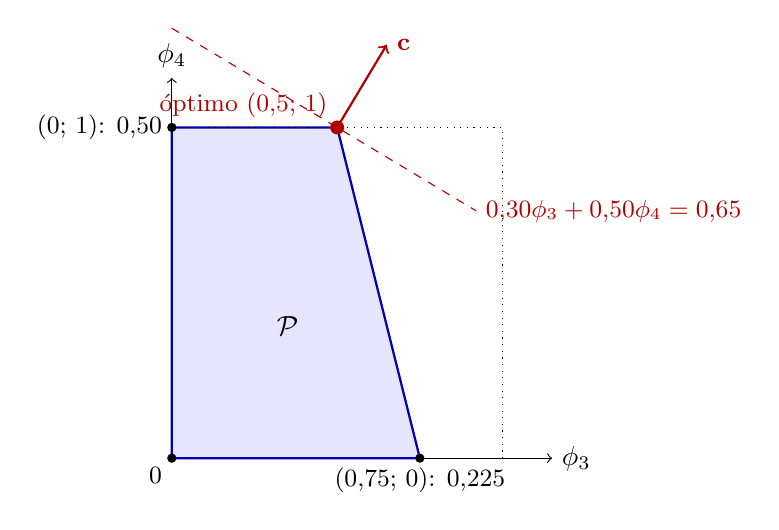
\begin{tikzpicture}[scale=4.2]
  \draw[->] (0,0) -- (1.15,0) node[right] {$\phi_3$};
  \draw[->] (0,0) -- (0,1.15) node[above] {$\phi_4$};
  \fill[blue!10] (0,0) -- (0.75,0) -- (0.5,1) -- (0,1) -- cycle;
  \draw[thick,blue!70!black] (0,0) -- (0.75,0) -- (0.5,1) -- (0,1) -- cycle;
  \draw[dotted] (1,0) -- (1,1) -- (0,1);
  \draw[red!70!black, dashed] (0,1.3) -- (0.92,0.748) node[right] {\small $0{,}30\phi_3 + 0{,}50\phi_4 = 0{,}65$};
  \draw[->,thick,red!70!black] (0.5,1) -- (0.5+0.15,1+0.25) node[right] {\small $\mathbf{c}$};
  \fill (0,0) circle (0.4pt) node[below left] {\small $0$};
  \fill (0.75,0) circle (0.4pt) node[below] {\small $(0{,}75;\,0)$: $0{,}225$};
  \fill (0,1) circle (0.4pt) node[left] {\small $(0;\,1)$: $0{,}50$};
  \fill[red!70!black] (0.5,1) circle (0.6pt) node[above left] {\small óptimo $(0{,}5;\,1)$};
  \node at (0.35,0.4) {$\mathcal{P}$};
\end{tikzpicture}
\caption{El PL~\eqref{eq:np_pl} restringido a $\phi_3$ y $\phi_4$ (con $\phi_1 = \phi_2 = 0$). La región factible es un
polígono; la recta de nivel del objetivo que lo toca más lejos en la dirección $\mathbf{c} = (0{,}30;\,0{,}50)$ lo
hace en un vértice. En cada vértice se indica el valor del objetivo.}
\label{fig:pl_np}
\end{figure}

La estructura de la solución no es casual: se activan los intervalos \emph{en orden decreciente de la razón}
$p_1(i)/p_0(i)$ hasta agotar el presupuesto $\alpha$, y a lo sumo un intervalo queda fraccionario (una sola
variable básica, porque hay una sola restricción además de las cotas). El multiplicador $\lambda = 7{,}5$ es la
razón de verosimilitud de ese intervalo: es el umbral. La Sección~\ref{sec:neyman_pearson} generaliza este
resultado a puntajes continuos.

\section{Aplicación 1: la función softmax}
\label{sec:softmax}

La regresión logística multinomial (Capítulo~\ref{cap:convexos}) calcula un puntaje lineal por clase,
$z_k = \vw_k^\top\vx + b_k$, y lo convierte en un punto del simplex $\Delta^{K-1}$. Por la
Proposición~\ref{prop:lineal_simplex}, maximizar el puntaje esperado $\mathbf{p}^\top\mathbf{z}$ sobre el simplex da un
vértice: la decisión dura $\argmax_k z_k$, que no es diferenciable. Si se agrega la entropía como término que
premia la incertidumbre, se obtiene una versión suave:
\begin{equation}
  \max_{\mathbf{p}}\ \sum_k p_k z_k - \sum_k p_k\log p_k \quad\text{s.a.}\quad \sum_k p_k = 1,\quad p_k \ge 0.
  \label{eq:softmax_problema}
\end{equation}

\begin{proposicion}
La solución única de~\eqref{eq:softmax_problema} es
\begin{equation}
  p_k^* = \operatorname{softmax}(\mathbf{z})_k = \frac{e^{z_k}}{\sum_{j=1}^K e^{z_j}}.
\end{equation}
\end{proposicion}
\begin{proof}
Se deja de lado por ahora la restricción $p_k \ge 0$. El Lagrangiano es
$\mathcal{L}(\mathbf{p}, \nu) = \sum_k p_k z_k - \sum_k p_k\log p_k + \nu\big(\sum_k p_k - 1\big)$, y
\[
  \frac{\partial\mathcal{L}}{\partial p_k} = z_k - \log p_k - 1 + \nu = 0
  \quad\Longrightarrow\quad p_k = e^{\nu - 1}\,e^{z_k}.
\]
La restricción $\sum_k p_k = 1$ fija $e^{\nu-1} = 1/\sum_j e^{z_j}$. La solución tiene todas las coordenadas
positivas, así que las restricciones $p_k \ge 0$ no están activas y por holgura complementaria sus multiplicadores
son nulos: no cambian nada. El objetivo es estrictamente cóncavo (la entropía lo es: su Hessiana es
$-\operatorname{diag}(1/p_k) \prec 0$) y el conjunto factible es convexo, así que el punto estacionario es el único
máximo global.
\end{proof}

Con un factor de temperatura $T > 0$ delante de la entropía, la solución es $\operatorname{softmax}(\mathbf{z}/T)$. Cuando
$T \to 0$ se recupera el vértice $\mathbf{e}_{k^*}$ (la solución del PL) y cuando $T \to \infty$, el baricentro.

\paragraph{Convexidad de la entropía cruzada.} La pérdida de un ejemplo de clase $y$ es
$-\log p_y = -z_y + \log\sum_j e^{z_j}$. Su gradiente y su Hessiana respecto de $\mathbf{z}$ son
\begin{equation}
  \nabla_{\mathbf{z}}(-\log p_y) = \mathbf{p} - \mathbf{e}_y,
  \qquad
  \nabla^2_{\mathbf{z}}(-\log p_y) = \operatorname{diag}(\mathbf{p}) - \mathbf{p}\mathbf{p}^\top.
  \label{eq:grad_ce}
\end{equation}
Para todo $\mathbf{v}$, $\mathbf{v}^\top(\operatorname{diag}(\mathbf{p}) - \mathbf{p}\mathbf{p}^\top)\mathbf{v} = \sum_k p_k v_k^2 - \big(\sum_k p_k v_k\big)^2$,
que es la varianza de $v$ bajo la distribución $\mathbf{p}$ y por lo tanto es $\ge 0$. La pérdida es convexa en
$\mathbf{z}$ y, como $\mathbf{z}$ es afín en los parámetros $(W, \mathbf{b})$, también lo es en ellos. El gradiente
$\mathbf{p} - \mathbf{e}_y$ (``predicción menos verdad'') es el mismo que se propaga hacia atrás en la última capa de la
CNN (Capítulo~\ref{cap:cnn}).

\section{Aplicación 2: el dual del SVM}
\label{sec:svm_dual}

\subsection{Primal}

Con etiquetas $y_i \in \{-1, +1\}$, un clasificador lineal decide con el signo de $f(\vx) = \vw^\top\vx + b$. La
distancia de un punto al hiperplano $f = 0$ es $|f(\vx)|/\lVert\vw\rVert$; si se normaliza para que los puntos más
cercanos cumplan $y_i f(\vx_i) = 1$, el \emph{margen} (ancho de la franja vacía) es $2/\lVert\vw\rVert$. Maximizar el
margen permitiendo violaciones $\xi_i$, penalizadas con un peso $C$, es el SVM de margen blando
\parencite{cortes1995}:
\begin{equation}
  \min_{\vw, b, \boldsymbol\xi}\ \frac12\lVert\vw\rVert^2 + C\sum_{i=1}^n\xi_i
  \quad\text{s.a.}\quad y_i(\vw^\top\vx_i + b) \ge 1 - \xi_i,\quad \xi_i \ge 0.
  \label{eq:svm_primal}
\end{equation}
Es un problema convexo (objetivo cuadrático convexo, restricciones afines) que cumple la condición de Slater:
el punto $\vw = \mathbf{0}$, $b = 0$, $\xi_i = 2$ satisface todas las desigualdades en forma estricta. Hay entonces
dualidad fuerte y las condiciones KKT caracterizan el óptimo.

\subsection{Lagrangiano y dual}

Con multiplicadores $\alpha_i \ge 0$ para la restricción de margen y $\mu_i \ge 0$ para $\xi_i \ge 0$:
\begin{equation}
  \mathcal{L} = \frac12\lVert\vw\rVert^2 + C\sum_i\xi_i - \sum_i\alpha_i\big[y_i(\vw^\top\vx_i + b) - 1 + \xi_i\big] - \sum_i\mu_i\xi_i.
\end{equation}
La estacionariedad respecto de las variables primales da
\begin{align}
  \frac{\partial\mathcal{L}}{\partial\vw} = 0 &\;\Rightarrow\; \vw = \sum_i\alpha_i y_i\vx_i, \label{eq:svm_w}\\
  \frac{\partial\mathcal{L}}{\partial b} = 0 &\;\Rightarrow\; \sum_i\alpha_i y_i = 0, \\
  \frac{\partial\mathcal{L}}{\partial\xi_i} = 0 &\;\Rightarrow\; \alpha_i = C - \mu_i \;\Rightarrow\; 0 \le \alpha_i \le C.
\end{align}
Reemplazando en $\mathcal{L}$, los términos en $b$ y en $\xi_i$ se cancelan y queda la función dual. El
\textbf{problema dual} es
\begin{equation}
  \max_{\boldsymbol\alpha}\ \sum_i\alpha_i - \frac12\sum_{i,j}\alpha_i\alpha_j\,y_i y_j\,\vx_i^\top\vx_j
  \quad\text{s.a.}\quad 0 \le \alpha_i \le C,\quad \sum_i\alpha_i y_i = 0.
  \label{eq:svm_dual}
\end{equation}

\subsection{Holgura complementaria y vectores soporte}

Las condiciones $\alpha_i\big[y_i f(\vx_i) - 1 + \xi_i\big] = 0$ y $\mu_i\xi_i = (C - \alpha_i)\xi_i = 0$ clasifican los
puntos según su margen funcional $m_i = y_i f(\vx_i)$ (Tabla~\ref{tab:svm_kkt}).

\begin{table}[ht]
\centering
\caption{Holgura complementaria en el SVM de margen blando.}
\label{tab:svm_kkt}
\begin{tabular}{lll}
\toprule
Multiplicador & Condición sobre $m_i = y_i f(\vx_i)$ & Interpretación \\
\midrule
$\alpha_i = 0$       & $m_i \ge 1$ & bien clasificado fuera del margen; no influye en $\vw$ \\
$0 < \alpha_i < C$   & $m_i = 1$   & vector soporte exactamente sobre el margen \\
$\alpha_i = C$       & $m_i \le 1$ & dentro del margen o mal clasificado; $\xi_i = 1 - m_i$ \\
\bottomrule
\end{tabular}
\end{table}

Por~\eqref{eq:svm_w}, $\vw$ es una combinación de los puntos con $\alpha_i > 0$, los \textbf{vectores soporte}. Los
demás se podrían eliminar del conjunto de entrenamiento sin cambiar la solución. Además, el sesgo se recupera de
cualquier vector soporte libre ($0 < \alpha_i < C$) a partir de $y_i(\vw^\top\vx_i + b) = 1$.

\subsection{Núcleos}

El dual~\eqref{eq:svm_dual} y la función de decisión $f(\vx) = \sum_i\alpha_i y_i\,\vx_i^\top\vx + b$ dependen de los
datos solo a través de productos internos. Reemplazándolos por un \emph{núcleo} $k(\vx_i, \vx_j) = \varphi(\vx_i)^\top\varphi(\vx_j)$
se obtiene un clasificador lineal en un espacio de atributos $\varphi(\vx)$, posiblemente de dimensión infinita,
sin calcularlo nunca explícitamente. El núcleo gaussiano (RBF), $k(\vx, \vx') = \exp(-\gamma\lVert\vx - \vx'\rVert^2)$,
es el que se usa en Bonn. Mientras la matriz $[k(\vx_i, \vx_j)]$ sea semidefinida positiva, el dual sigue siendo
convexo y todo lo anterior vale.

En el Capítulo~\ref{cap:convexos} se resuelve este problema para separar el set E del set D de Bonn y se verifican
numéricamente cada una de estas condiciones.

\section{Aplicación 3: el lema de Neyman-Pearson}
\label{sec:neyman_pearson}

\subsection{Planteo}

En el problema de detección de la Sección~\ref{sec:hipotesis} se busca decidir entre $H_0$ (sin crisis) y $H_1$
(crisis) a partir de los atributos $\vx$ de una ventana, con densidades $p_0(\vx)$ y $p_1(\vx)$. Un test es una
función $\phi(\vx) \in [0,1]$, la probabilidad de declarar crisis. Sus dos medidas de desempeño son
\begin{equation}
  P_D(\phi) = \int\phi(\vx)\,p_1(\vx)\,d\vx \quad\text{(detección, sensibilidad)},
  \qquad
  P_{FA}(\phi) = \int\phi(\vx)\,p_0(\vx)\,d\vx \quad\text{(falsa alarma, } 1 - \text{especificidad)}.
\end{equation}
No se pueden mejorar las dos a la vez. En un monitor de crisis lo que se fija de antemano es cuántas falsas
alarmas se toleran, así que el problema es
\begin{equation}
  \max_{\phi}\ P_D(\phi) \quad\text{sujeto a}\quad P_{FA}(\phi) \le \alpha.
  \label{eq:np_problema}
\end{equation}
Es la versión continua del PL~\eqref{eq:np_pl}: objetivo y restricción son lineales en $\phi$, y $0 \le \phi \le 1$.

\subsection{El lema}

\begin{teorema}[Neyman-Pearson \parencite{neyman1933}]
\label{teo:np}
Sea $\lambda \ge 0$ y el test
\begin{equation}
  \phi^*(\vx) =
  \begin{cases}
    1 & \text{si } p_1(\vx) > \lambda\,p_0(\vx), \\
    \gamma & \text{si } p_1(\vx) = \lambda\,p_0(\vx), \\
    0 & \text{si } p_1(\vx) < \lambda\,p_0(\vx),
  \end{cases}
  \label{eq:np_test}
\end{equation}
con $\lambda$ y $\gamma \in [0,1]$ elegidos para que $P_{FA}(\phi^*) = \alpha$. Entonces $P_D(\phi^*) \ge P_D(\phi)$
para todo test $\phi$ con $P_{FA}(\phi) \le \alpha$.
\end{teorema}
\begin{proof}
Sea $\phi$ un test con $P_{FA}(\phi) \le \alpha$. En todo punto se cumple
\[
  \big(\phi^*(\vx) - \phi(\vx)\big)\big(p_1(\vx) - \lambda\,p_0(\vx)\big) \ge 0:
\]
donde $p_1 > \lambda p_0$, $\phi^* = 1 \ge \phi$; donde $p_1 < \lambda p_0$, $\phi^* = 0 \le \phi$; y donde son
iguales el producto es cero. Integrando,
\[
  P_D(\phi^*) - P_D(\phi) \;\ge\; \lambda\big(P_{FA}(\phi^*) - P_{FA}(\phi)\big) = \lambda\big(\alpha - P_{FA}(\phi)\big) \;\ge\; 0. \qedhere
\]
\end{proof}

\subsection{Lectura con multiplicadores de Lagrange}

El test~\eqref{eq:np_test} es exactamente lo que dan las condiciones KKT de~\eqref{eq:np_problema}. El Lagrangiano es
\begin{equation}
  \mathcal{L}(\phi, \lambda) = P_D(\phi) - \lambda\big(P_{FA}(\phi) - \alpha\big)
  = \int\phi(\vx)\,\big[p_1(\vx) - \lambda\,p_0(\vx)\big]\,d\vx + \lambda\alpha,
  \qquad \lambda \ge 0.
\end{equation}
Para $\lambda$ fijo, maximizarlo en $\phi \in [0,1]$ es trivial punto a punto: $\phi = 1$ donde el integrando es
positivo y $\phi = 0$ donde es negativo. Eso es~\eqref{eq:np_test}, y equivale a comparar la \textbf{razón de
verosimilitud} $\Lambda(\vx) = p_1(\vx)/p_0(\vx)$ con el umbral $\lambda$. Las demás condiciones KKT completan la
lectura:
\begin{itemize}
  \item \textbf{Holgura complementaria:} $\lambda\,(P_{FA} - \alpha) = 0$. Como bajar el umbral nunca reduce $P_D$, si
        sobrara presupuesto de falsas alarmas convendría usarlo: la restricción está activa ($P_{FA} = \alpha$) y
        $\lambda > 0$.
  \item \textbf{Sensibilidad:} por~\eqref{eq:sensibilidad}, $\lambda = dP_D^*/d\alpha$: el multiplicador dice cuánta
        detección se gana por cada unidad extra de falsas alarmas que se acepta.
  \item \textbf{Pendiente de la curva ROC:} si el test es $s(\vx) > \tau$ con densidades del puntaje $q_1, q_0$, entonces
        $dP_D/d\tau = -q_1(\tau)$ y $dP_{FA}/d\tau = -q_0(\tau)$, de modo que
        \begin{equation}
          \frac{dP_D}{dP_{FA}} = \frac{q_1(\tau)}{q_0(\tau)} = \lambda.
          \label{eq:pendiente_roc}
        \end{equation}
        En el punto de operación óptimo, la pendiente de la curva ROC (Capítulo~\ref{cap:metricas}) es igual al
        multiplicador. Con $\alpha$ muy chico el punto de operación está en el extremo izquierdo de la curva, donde la
        pendiente es grande: por eso importa tanto esa zona y por eso la ROC se grafica con el eje horizontal en
        escala logarítmica.
\end{itemize}

\subsection{De la teoría a la práctica}

Las densidades $p_0$ y $p_1$ son desconocidas, de modo que el test óptimo no se puede calcular directamente. Se usa
que \emph{cualquier función estrictamente creciente de la razón de verosimilitud} da el mismo test (con otro umbral).
La regresión logística modela justamente
\begin{equation}
  s(\vx) = \vw^\top\vx + b \approx \log\frac{P(H_1\mid\vx)}{P(H_0\mid\vx)} = \log\Lambda(\vx) + \log\frac{\pi_1}{\pi_0},
\end{equation}
que es creciente en $\Lambda$. El peso por clase (\texttt{class\_weight="balanced"}) solo cambia la constante
$\log(\pi_1/\pi_0)$, no el orden de los puntajes. La salida de la CNN, antes de la sigmoide, se interpreta igual.

El umbral se elige entonces sobre el puntaje y no sobre $\Lambda$. Como $P_{FA}(\tau) = P(s > \tau \mid H_0)$, la
condición $P_{FA} = \alpha$ dice que \emph{$\tau$ es el cuantil $1 - \alpha$ de la distribución del puntaje sin crisis}.
Se estima con el cuantil empírico sobre las $n_0$ ventanas sin crisis de un conjunto que no se usa para evaluar:
\begin{equation}
  \hat\tau = s_{(\lceil(1-\alpha)\,n_0\rceil)},
  \label{eq:umbral_np}
\end{equation}
el estadístico de orden correspondiente (en el código, \texttt{np.quantile(..., method="higher")}). En el trabajo
se usa $\alpha = 10^{-3}$: con ventanas de 4 s hay 900 por hora, así que $\alpha$ corresponde a unas 0,9
ventanas falsas por hora antes del suavizado. El conjunto de calibración es el de los pacientes de entrenamiento
en el esquema LOPO, y el paciente de validación (chb01) en la partición fija.

\begin{observacion}
\label{obs:np_supuesto}
El lema garantiza $P_{FA} = \alpha$ solo si la distribución del puntaje sin crisis es la misma en la calibración y
en el uso. Entre pacientes distintos eso no se cumple: en el Capítulo~\ref{cap:convexos} la tasa real de falsas alarmas
en el paciente nuevo va de 0 a 4,6 por hora con el mismo umbral. La calibración por paciente
(Sección~\ref{sec:modelo}) reduce ese desajuste, pero no lo elimina.
\end{observacion}
